\chapter{Three plastic network prototypes for DYNAP-SE1 chip}
\label{ch:EXAMPLES}

 This chapter presents three network examples implemented on the DYNAP-SE1 chip, combining all of the elements introduced in the previous chapters.
 These examples show how, by combining the principles of neuron clustering (i.e. space averaging), population coding and feedback inhibition in the network with online Hebbian plasticity, one can obtain biologically observed and functionally relevant behaviour.

The first network (see Section~\ref{sec:unsupervised_WTA_map}) is a simplest \emph{relational network}~\cite{Diehl_Cook16}, except the relation is not imposed on the system: competitive interaction of Hebbian learning rule with inhibition and weight regularization creates robust continuous maps through just exploratory behaviour. This prototype network demonstrates the unsupervised formation of a mapping between two population-coded variables~\cite{Song_Abbott01}.

Section~\ref{sec:Caterina's_setup} introduces a fully integrated sensorimotor control loop, with the DYNAP-SE1 and the computer-in-the-loop R-STDP plasticity framework working online in conjunction with the real DAVIS event-based camera and a physical motor to move the camera towards the target. The work towards completion of that system inspired some of the design decisions for the chip-in-the-loop framework.

Finally, the Section~\ref{sec:delay_lines} makes a step from the rate-based population codes and demonstrates time-sensitive, or timing-dependent, learning on a neuromorphic chip. The network learns to discriminate spatiotemporal patterns, and the nature of the R-STDP mechanism fits perfectly for an efficient asynchronous implementation for the task. Specifically, this network architecture was born out of trying to answer the question of how one could make a spiking network discriminate clockwise and counter-clockwise rotation of some image, doing a full 360-degree turn and returning to the initial position. 

These examples should be seen as computational building blocks, demonstrating behaviour where every component introduced in the previous chapters is essential. All while dealing with built-in unit variability of the chip and very low individual weight precision.


\newpage
\section{Unsupervised map formation between sWTA networks}
\label{sec:unsupervised_WTA_map}

The first dynamic network example demonstrates a process of an unsupervised mapping formation between the two one-dimensional variables, encoded with population codes in the two one-dimensional \ac{sWTA} populations A and B. A pool of plastic connections from A to B creates a unidirectional transformation projection. In the presence of reverse connections (i.e. from B to A) this would become a \emph{relation}~\cite{Diehl_Cook16}, although to simplify the process of learning convergence, it was omitted.

The experiment is set up as follows: two \ac{sWTA} populations, A and B, with non-equal sizes $N_A$ and $N_B$ are configured and tuned similar to the Section~\ref{sec:sWTA}, such that (i) the population coded input is represented with its sharpened version; (ii) in the absence of input the population activity bump is sustained through sufficient recurrent excitation balanced with feedback inhibition; and (iii) the uniform feedback inhibition ensures that only one population code can exist at a time.

Population A is driven with a population-coded input. The input bump position is constant for the duration of one trial with a length of one second. Population B is driven through the set of plastic R-STDP connections (see Figure~\ref{fig:Unsupervised_WTA_mapping}). The matrix is initialized uniformly while maintaining the rule of the fixed total weight sum for every postsynaptic neuron (Eq.~\ref{eq:fixed_weight_sum}) to keep the excitability of the population B under control and ensure the neurons in population B remain sensitive to the same fraction of population A (the input space).

\begin{figure}[h]
  \centering
    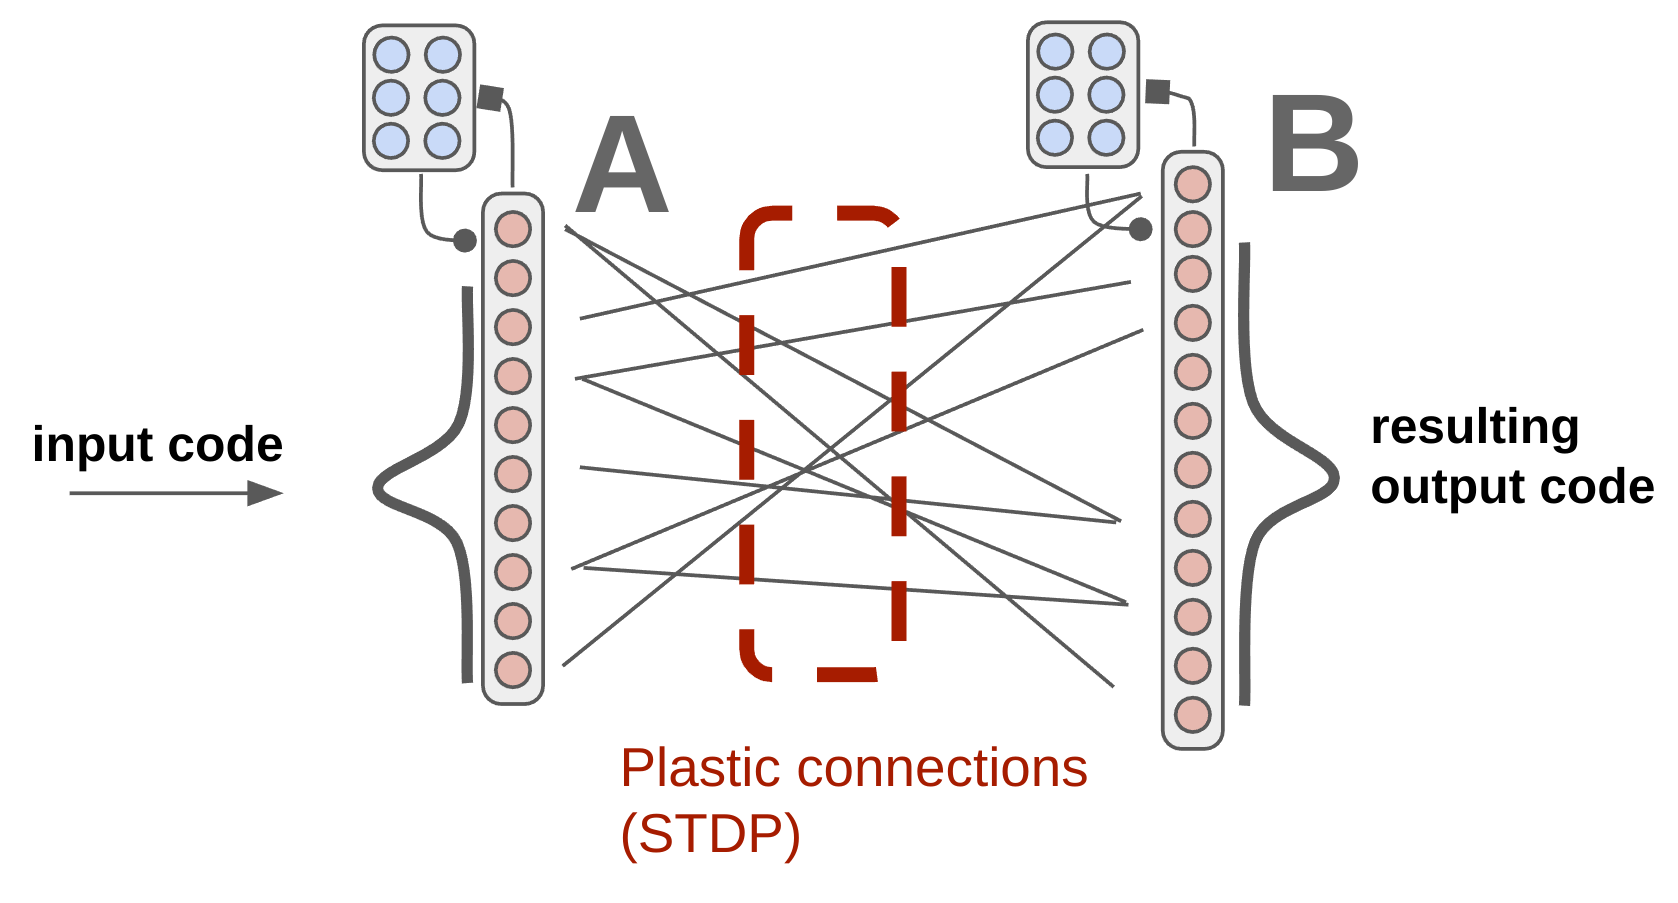
\includegraphics[width=\linewidth]{img/chapter5/Unsupervised_WTA_mapping.png}
    \caption[Unsupervised WTA mapping formation.]{Unsupervised WTA mapping formation experiment. Two sWTA populations A and B are connected with a pool of plastic feedforward R-STDP synapses. Inputs in the form of population codes are presented consecutively to population A at random locations for the duration of 1 second each. Activity in population B is purely input-driven, while the input weight sum of every neuron in B is clamped to a uniform fixed value. The parameter tuning in B ensures that activity can only exist in the form of a single population bump, inhibiting any non-local activity.}
  \label{fig:Unsupervised_WTA_mapping}
\end{figure}

After the presentation of one input, the ``reward'' signal (see Section~\ref{sec:RSTDP}) is sent to the plastic connections module to process the current state of the eligibility traces and to calculate and apply the weight updates. The reward signal is only used here for sparse regular hardware connection updates and set to a constant amplitude of $A_{da}$, as the matrix update on the chip requires time to be applied, as discussed in Section~\ref{sec:RSTDP}. For the duration of the matrix update the input to A is still presented for continuity.

\begin{figure}[h]
  \centering
    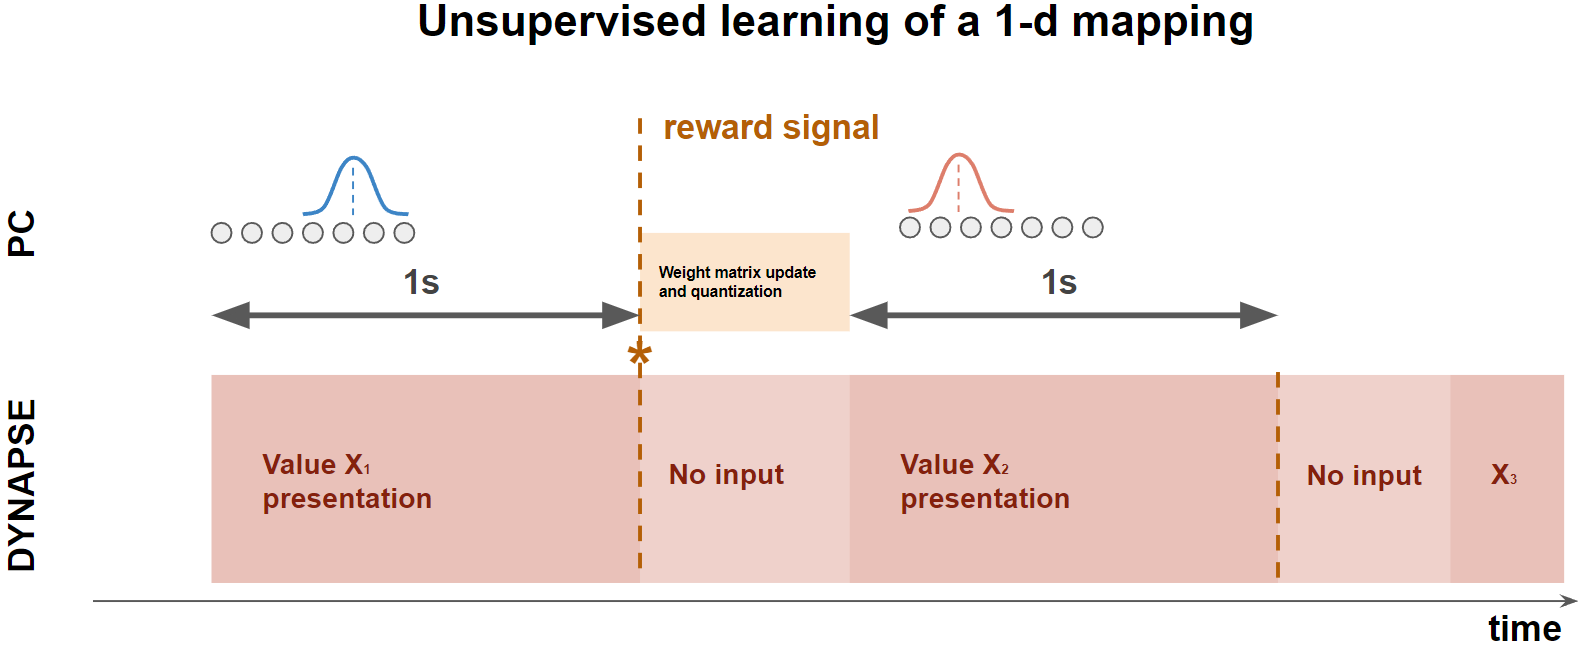
\includegraphics[width=\linewidth]{img/chapter5/unsupervised_mapping_training.png}
    \caption[Unsupervised mapping training protocol]{Unsupervised mapping training protocol. Input value $A=X_1$ encoded with a Poisson rate population code is sent to population A (shown in Fig.~\ref{fig:Unsupervised_WTA_mapping}) for the duration of one second, while it activates some bump-shaped activation in population B. The PyEPC module is active at all times, integrating events and continuously updating the eligibility traces of all possible pairs of neurons between A and B. After the presentation of the input $X_1$, the reward signal is sent to the EPC module to initiate the matrix update based on the snapshot of the values of the eligibility traces. After the update is completed, a new random value of A is presented.}
  \label{fig:Unsupervised_mapping_training}
\end{figure}



The next value of A is presented immediately after the plasticity update is finished. The values of A are sampled randomly to avoid correlations between neighbouring inputs.

The result of running the experiment is a self-organizing continuous diagonal mapping between A and B (see Figure~\ref{fig:unsupervised_mapping_examples}. Due to the non-deterministic nature of the chip, the forming diagonal may be shifted or even inverted, but the dynamics of the weight evolution always create a consistent structure regardless of the relative sizes of the A and B populations.

The only exception is the case of a discontinuity in a growing diagonal segment of a weight matrix, where one part happens to be along the main matrix diagonal and another is reversed. This might happen if the amplitudes of the parameters contributing to weight changes (i.e. learning rates) are too high. This causes the weights to quickly form small structured diagonal regions responsible for the neighbouring states of A and B, but the symmetry in the system would forbid migration of a such formed piece to connect with the other one, as the movement of a weight cluster in one direction is as probable is in the opposite one creating no bias to ``polarize'' the forming structure and force it to connect the gaps.

\begin{figure}[b!]
    \begin{subfigure}{.45\textwidth}
        \centering
        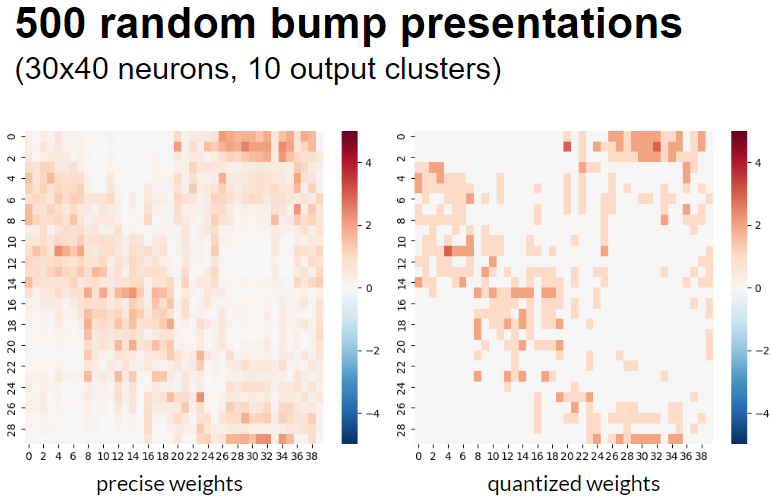
\includegraphics[width=\linewidth]{img/chapter5/unsupervised_mapping_500_smaller.png}
        \caption{}
        \label{fig:unsupervised_mapping_example_smaller}
    \end{subfigure}
    \hfill
    \begin{subfigure}{.44\textwidth}
        \centering
        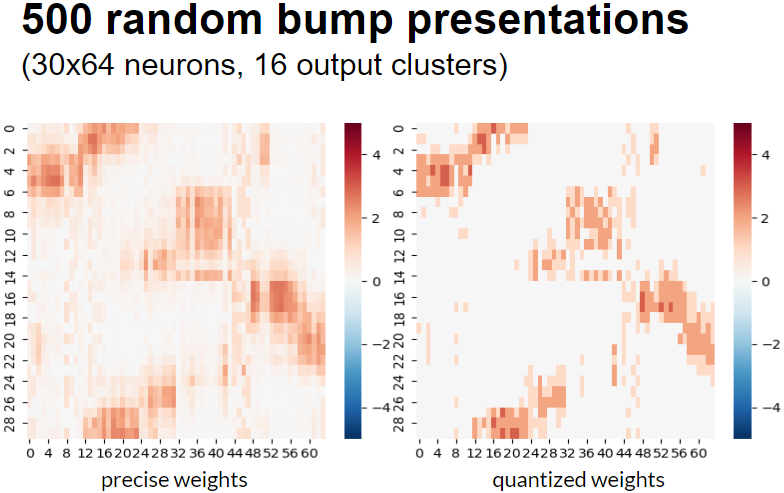
\includegraphics[width=\linewidth]{img/chapter5/unsupervised_mapping_500_bigger.png}
        \caption{}
        \label{fig:unsupervised_mapping_example_bigger}
    \end{subfigure}
    \caption[Unsupervised mapping formation examples]{Unsupervised mapping formation examples}
    \label{fig:unsupervised_mapping_examples}
\end{figure}

Notably, this behaviour is reported for similar networks in simulation when enabling STDP between the sWTA structures~\cite{Song_Abbott01} in a model for cortical selectivity remapping.

Crucial for the process of mapping convergence is the joint effect of Hebbian firing correlation reinforcement with the two types of competition: the \ac{sWTA} and the fixed total input weight sum (see Eq.~\ref{eq:fixed_weight_sum}). The intuition for their interplay is the following. STDP increases the weights between the neurons that are active simultaneously in both populations A and B. Since sWTA ensures only a spatially local group of neurons (spanning multiple neighbouring clusters at most) can be active at a time, any neuron in population B is active together with a bump-shaped activation pattern of neurons in A. At the same time, as the input weight sum is fixed, with many presentations of various inputs in A, the presynatic weights of this neuron in B would either (a) spread thin and therefore yield no preference to input, or (b) for a bump-shaped receptive field located somewhere in population A. Finally, the competition between neurons in population B won't let them have fully overlapping receptive fields, as that region of A would drive both of them equally, leading to one of them winning over the other eventually. Overall, this interaction of mechanisms ensures formation of a well-distributed mapping.

An important note here is that the proximity metric is embedded in the sWTA networks: both A and B are ring attractors with clusters of excitatory neurons connected to their nearest neighbours. This imposes metric structure onto the matrix automatically. A more interesting experiment would be enabling plasticity within the sWTA populations, to first form the internal representations of the inputs. However, if we keep the demand that we would like to preserve the proportions of the recurrent and excitatory-to-excitatory connections, some metric would still form in the within the populations A and B, and sorting the neurons by correlating their activity could let us determine the neighbouring ones and give us very similar visualization.

The competition that enforces this distributed mapping is the same as the one demonstrated by Peter Diehl \cite{Diehl_Cook15} to be able to efficiently learn to classify MNIST unsupervised, only through input presentations. Notably, although in simulation, for robustness, he used 100 output neurons, having 10 neurons per class, which is in line with the space averaging considerations.\\

The direct function of such a building block is any linear mapping between two internal state variables representing, for example, joint angles of a robotic arm. Multiple connections like this with various value limitations could form a network of relations between multiple joints, with all those mappings continuously refining their precision through plasticity based on sensory feedback from the environment. Following the example of robotics, such online refinement for motor actions would reduce the need for expensive precise electronics and enable the use of fast-reacting muscle-like flexible actuators. These results are also consistent with the concept of learning inverse kinematics of motor control through babbling~\cite{Zhao_etal20}.

Finally, the notable property of this network prototype is its size, as usually thousands of neurons are often used for such structures to work robustly~\cite{Diehl_Cook16}, while here the sizes of A and B populations varied between 20 and 100 neurons, while having the fixed 10-20\% variability of parameters, sparse connectivity matrix and the low weight precision (no more than 2-bit).

\newpage
\section{Visual target following in a closed neuromorphic sensorimotor loop}
\label{sec:Caterina's_setup}

This work has been done together with an MSc student Caterina Caccavella as her semester project, serving as the first testbench for the plasticity module, building on top of Nicoletta Risi's DAVIS-to-DYNAP-SE1 hardware setup~\cite{Risi_etal21}.

This section presents a fully embodied neuromorphic agent with the goal of learning active target following through reinforcement learning, consisting of the DYNAP-SE1 R-STDP learning framework embedded into a closed sensorimotor loop with neuromorphic hardware peripherals (see~\ref{fig:camera_closed_loop_setup_photo}). The task of the agent is to learn to move the event-based DAVIS camera to follow a lit-up target through a positive reinforcement signal.

\begin{figure}[h]
  \centering
    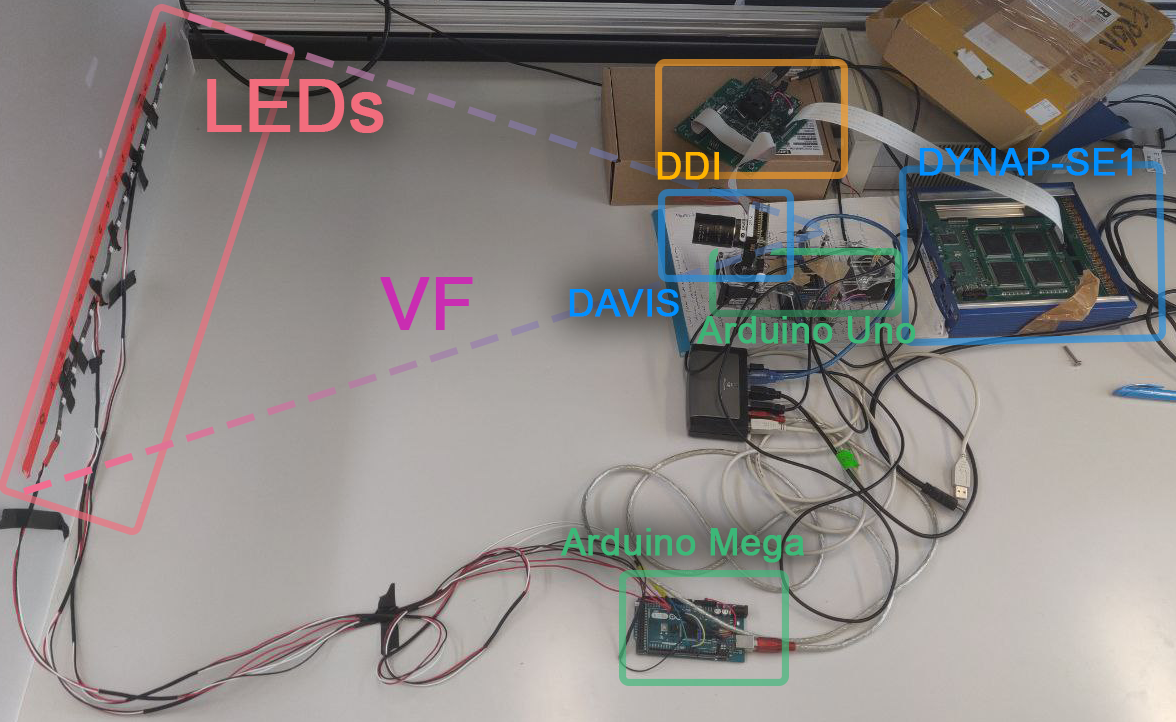
\includegraphics[width=\linewidth]{img/chapter5/Caterinas_setup.png}
    \caption[Closed loop setup for the DVS following task photo]{Closed loop setup}
  \label{fig:camera_closed_loop_setup_photo}
\end{figure}

The sketch in Figure~\ref{fig:camera_closed_loop_setup_sketch} shows the full processing pipeline. The Arduino-controlled LED strip activates rapid blinking of one of the lights as a target. That generates events within the camera's sensor. Through the DAVIS-to-DYNAP-SE1 (DDI) interface~\cite{Risi_etal21} the events are then streamed onto the DYNAP-SE1 board, where they activate an input WTA population ($N_{in}$). The output population $N_{out}$ is another (smaller) WTA population connected to the input through a pool of plastic R-STDP connections, responsible for selecting whether the camera should rotate left, right or remain still. The most active cluster in $N_{out}$ is determined digitally through the spike count, and the corresponding action is applied to the stepper motor through the Arduino controller, rotating the camera. The plastic weights between the input and the output populations are initialized random and evolve through trial and error in presence of the reward signal.

\begin{figure}[h]
  \centering
    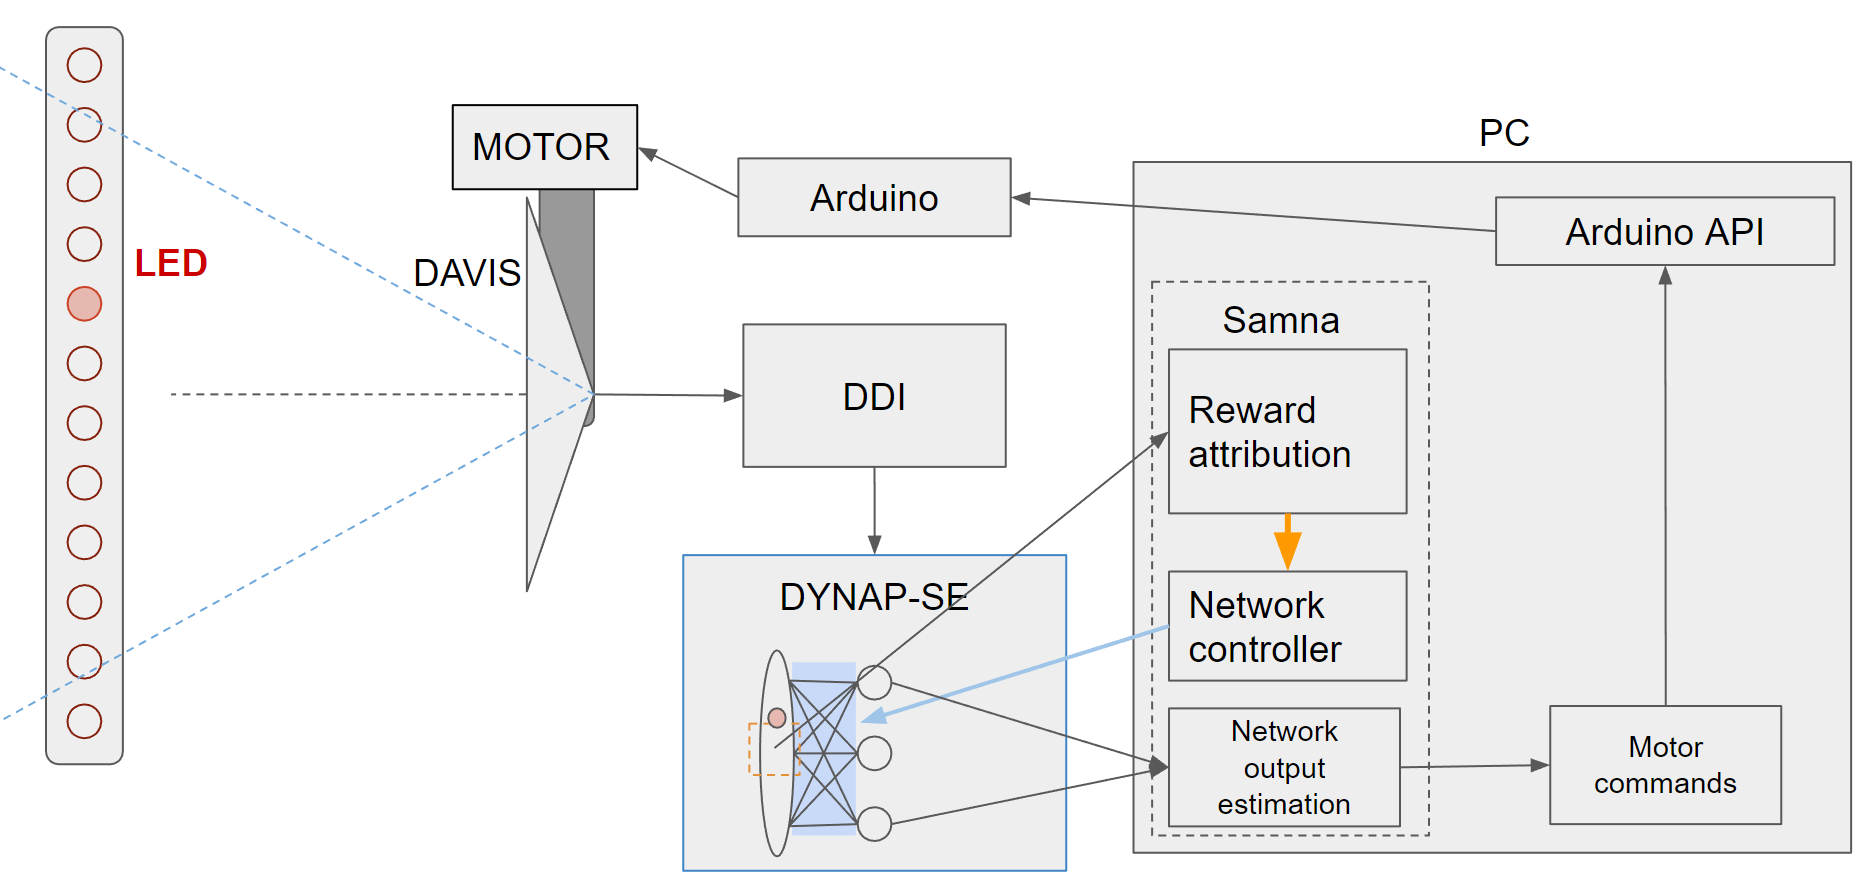
\includegraphics[width=\linewidth]{img/chapter5/Caterinas_setup_sketch.png}
    \caption[Closed loop setup for the DVS following task architecture sketch]{Setup sketch for the agent learning to follow the target by actively moving the camera. The target on the LED strip is registered by the DAVIS camera, feeding the events onwards to DYNAP-SE1 chip through the DDI module, performing downsampling of the input image from 320 to just 16 pixels wide. The plastic network on DYNAP-SE1 makes the decision for the motor command that is registered by the PC filter and transmitted to the stepper motor on which the DAVIS camera is mounted.}
  \label{fig:camera_closed_loop_setup_sketch}
\end{figure}

The reward signal is generated when the target is in the fovea (center) of the camera's visual field, reinforcing the last actions that led to the correct orientation towards the camera.

As the DAVIS cameras react to changes in the scene, we also had to implement the input suppression mechanism for the duration of the camera rotation, similar to the saccadic suppression found in biological visual systems, by shutting down the activity in the input layer of the network with the neuron time constant bias.\\

The trials were initialized with the camera centered and one of the LEDs illuminated (random for every trial). After the activity evaluation period, the motor moved the camera according to the most active neuron in the output population. After a series of steps the camera either focused on the target or exceeded the maximum number of saccades. In the case of successful trial, the reward signal was sent. Note that the R-STDP ran continuously for all of the experiments, meaning that long enough eligibility traces could remain non-negligible for the duration of multiple saccades, as a memory of the most recent actions that would be all reinforced if the last one is successful.

Additional algorithmic actions had been added in case no activity arrives to the camera (i.e. in case the target is out of the field of view of the camera): it was forced to perform rotation towards the center state.\\

\begin{figure}[h!]
  \centering
    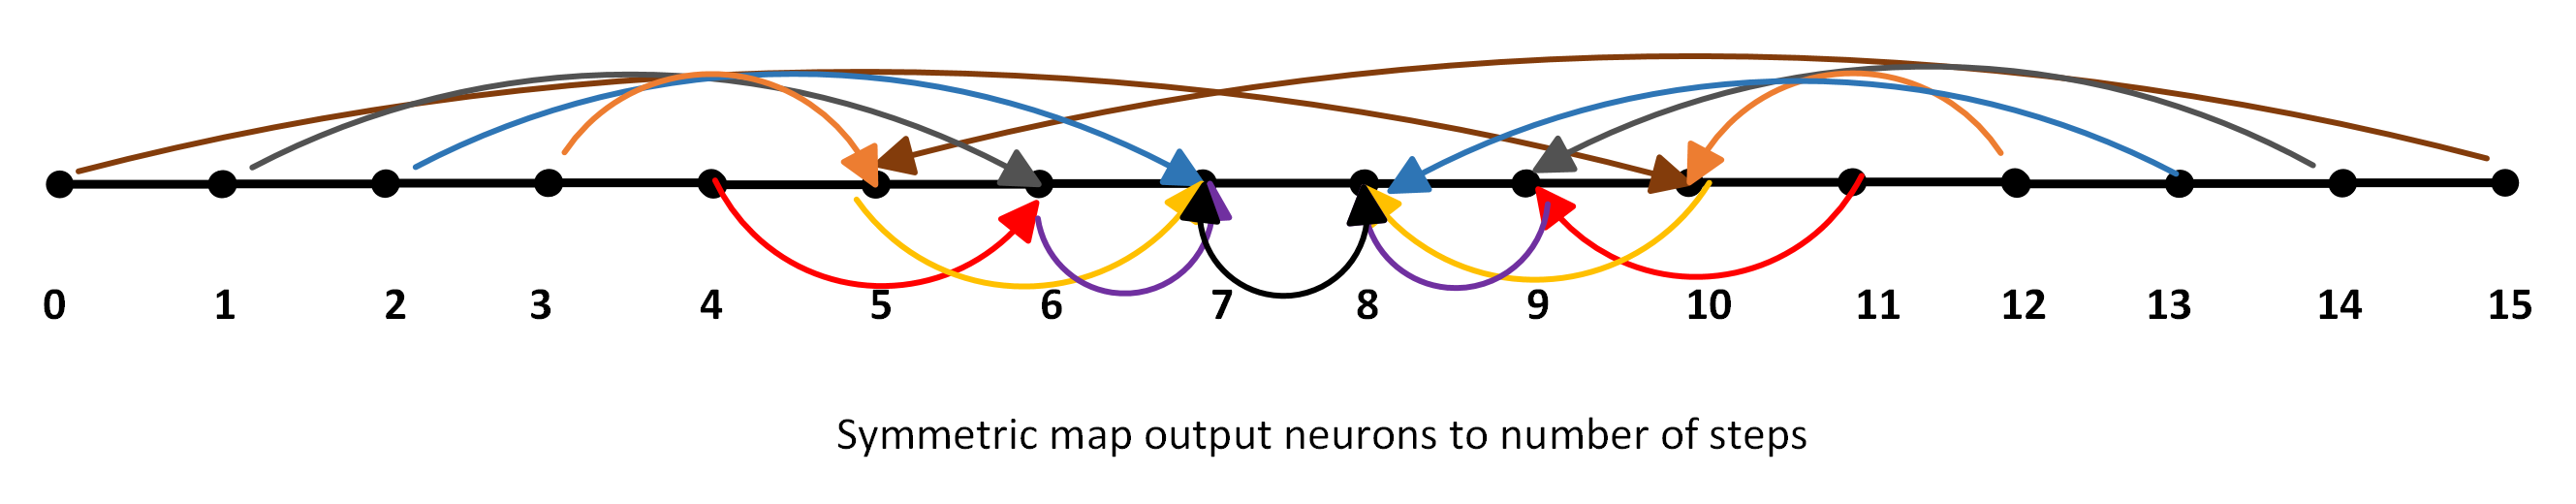
\includegraphics[width=\linewidth]{img/chapter5/camera_motor_map.png}
    \caption[Camera motor map]{An example of a motor map for rotating the camera a set amount of steps based on the action selected indicated by the most active output cluster. The possible actions include small moves of a few steps as well as long jumps almost across the entire visual field of the camera. The selection of the motor map drastically impacts the successful convergence of learning.}
  \label{fig:camera_motor_map}
\end{figure}

We found that convergence of learning depends widely on the motor action map, i.e. for the cases where the output population has only 3 output clusters ("move left", "hold still", "move right"), or more ("move $X_1$ steps to the left", "move $X_2$ steps to the left", ... , etc. See Figure~\ref{fig:camera_motor_map}). The more detailed motor map has to deal with overshooting the target and ideally learn to jump to the target in only one saccade (i.e. one action). With a flat or linear map we would expect to see a diagonal on the connectivity matrix, similar to a vector field forming in a Morris maze R-STDP task~\cite{Vasilaki09}. In practice, it is hard to say which map works best with the experience we had, but clearly the saccades that are both too short or too long results in the network failing to learn anything.\\

Unfortunately, we only managed to assemble the setup and get some preliminary results for the time being, as the challenge with had been mostly engineering. From the scientific point of view, however, we noticed some tendencies that could be addressed within the learning framework. For instance, despite the regularization mechanisms described above, the network tended to find only a couple of solutions that work and stick to them, meaning that the exploratory behaviour was not prominent enough (similar effect had been observed when we tried reproducing a spike based foraging agent~\cite{Sanda_etal17}). We tried introducing randomized exploratory actions, similar to Deep Q ANN training, but that resulted in the camera getting lost rather than expanding the connectivity map.

One training consideration worth exploring comes from machine learning RL, which is a more careful reward function choice. It is known that reward function profile defines convergence of learning for RL tasks such as Atari games.\\

To conclude, we can confirm that continuous learning is indeed a complex discipline. The challenges we faced, however, are on the computation side rather than architectural, proving that such a closed-loop setup does function and, with an updated training setting, would definitely function correctly.

\newpage
\section{Temporal pattern recognition learning}
\label{sec:delay_lines}

This network prototype revisits the concept of delay lines (or synfire chains)~\cite{Abeles91, Diesmann_etal99, Cariani_etal22} and proposes a spiking readout trained with a reward-gated STDP learning rule (the reward signal, however, serves only as a regular update signal for the external plasticity controller, so the network training should not be confused with any form of reinforcement learning).
%\dz{Briefly introduce common approaches to learning temporal sequences (go through the pool of saved references). Use the review of Cariani and Baker 2022~\cite{Cariani_etal22}.}

By using the delay lines, we can convert the time dimension of the input signal into spacial (or ``neural''), allowing a readout that listens to all of the neurons in the entire network of the delay lines to recognize (spatio-) temporal patterns. With the signal sequence moving along the delay lines, coincidence detection through STDP makes the readout form spatial receptive fields detecting specific sequences. As previously discussed, contrary to many other strategies for encoding time-varying inputs with spikes, the delay lines allow the representation of the temporal input information with uniform precision across the buffer (or "working memory"), i.e. without any discounting of the least recent information.

This means that such a network can be trained to classify multi-channel temporal sequences with overlapping sections, which other encoding methods, like \ac{TTFS} would fail to capture~\cite{Auge_etal21}. The perfect example of such a task is distinguishing between the full clockwise and counterclockwise rotations of a clock hand. Assuming we encode the hand motion in a \ac{DVS}-like event-based fashion (so that the edges of the moving object generate events from the respective pixels), when integrated across the full duration, both sequences would produce the exact same pixel spiking statistics. \ac{TTFS} approach would also be troubled by the beginning and the ending frames being identical. Indeed, there could be some more elaborate \ac{TTFS} detectors for the first encounters of specific temporal features, but very quickly, they become very dependent on the information format, as all of the information past the detection point is discarded.

\begin{figure}[h!]
  \centering
  \begin{subfigure}{0.7\textwidth}
    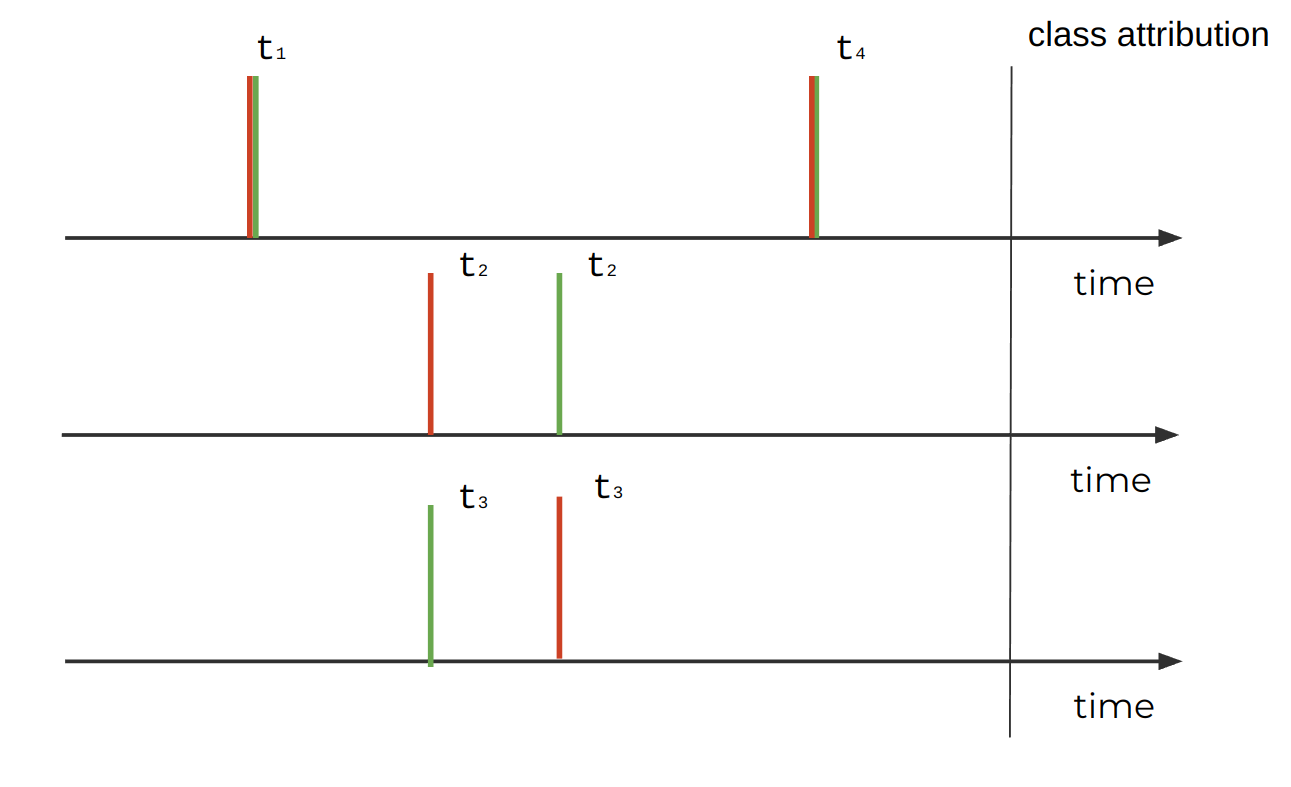
\includegraphics[width=\linewidth]{img/chapter3/temporal_pattern_task.png}
    \caption{}
  \end{subfigure}
    \caption[Temporal pattern classification task]{Temporal pattern classification task. Two patterns of spikes (red and green) have the same beginning and ending, but the second and third spikes are on different channels. The decoder should be able to extract and classify the difference between the patterns correctly.}
  \label{fig:temporal_pattern_task}
\end{figure}

\begin{figure}[h!]
  \centering
  \begin{subfigure}{.9\textwidth}
    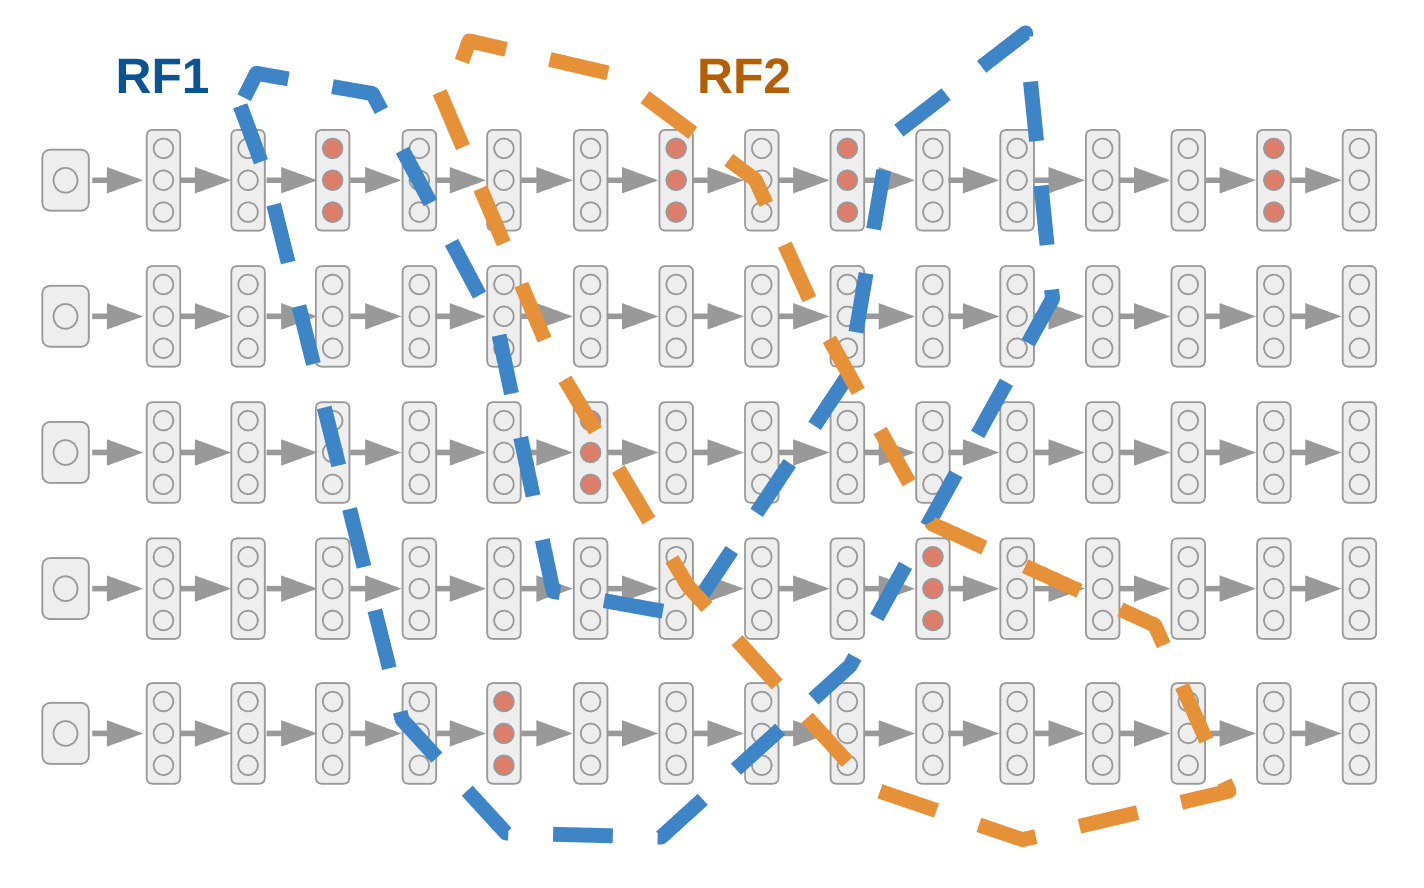
\includegraphics[width=\linewidth]{img/chapter3/neural_sheet_sketch.png}
    \caption{}
  \end{subfigure}
    \caption[Neural sheet sketch with receptive fields]{A sketch illustration of a neural sheet formed by multiple delay chains, with one per input channel. Under the condition that the pulse propagation speed is constant for every chain, the temporal structure of the input is converted to a spatial dimension, with the sheet length and the propagation speed defining the temporal window. Having a 2D representation, a spatiotemporal classifier would now just be a regular 2D receptive field over this sheet, as shown by examples RF1 and RF2. This decoding approach would process overlapping temporal sequences correctly.}
  \label{fig:neural_sheet_sketch}
\end{figure}

The delay line encoding avoids these drawbacks by preserving the input encoding as long as the memory time interval allows, with the memory capacity linearly scaling with the network size.

Another benefit of this network architecture is native hardware compatibility, as it does not rely on complex time-processing machinery like variable synaptic delays~\cite{Izhikevich06a}, implementation of which \emph{in silico} would increase the chip design complexity by an order of magnitude.

Finally, since the decoding deals with reacting to precise spike times from specific neurons, \ac{STDP}-based learning fits this framework very naturally, enabling efficient asynchronous and highly parallel learning.

Indeed, the plasticity part introduced is implemented off-chip, but it demonstrates the fundamental direction for circuit design in the future.


\subsection{Network architecture and experiment design}

The proposed network is shown in Figure~\ref{fig:RSTDP_temporal_recognition_prototype}. The network consists of multiple delay lines, one per input channel, receiving independent spike trains and converting interspike intervals into gaps between the activated units of the delay chains. The readout population listens to the entire delay line sheet with plastic all-to-all pool of connections. For the on-chip implementation, this is done with the chip-in-the-loop RSTDP EPC framework, treating the delay line block as a presynaptic population and the readout as postsynaptic, tracking the pairwise activity of all of these neurons and using the regular ``reward'' signal to apply cumulative weight updates.


\begin{figure}[h]
  \centering
    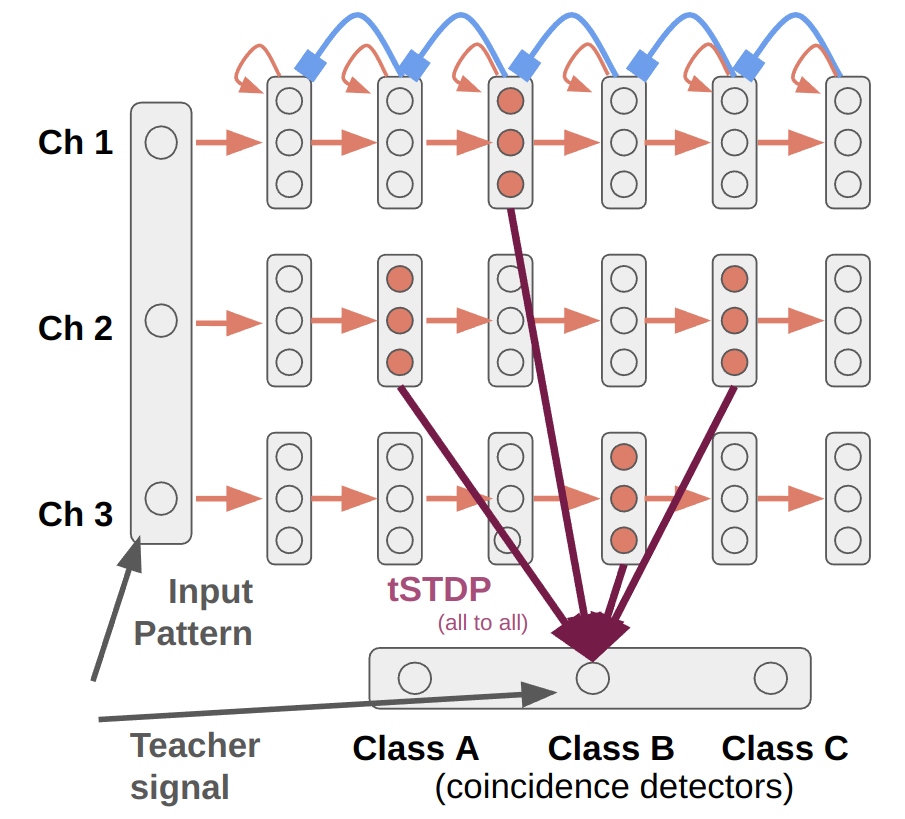
\includegraphics[width=.8\linewidth]{img/chapter5/RLSTDP_temporal_recognition_prototype.png}
    \caption[RSTDP temporal pattern recognition prototype]{RSTDP temporal pattern recognition prototype}
  \label{fig:RSTDP_temporal_recognition_prototype}
\end{figure}

During training, the output population clusters are activated by the teacher signal, providing the label for the class of the sequence presented.

The network we used consisted of 3 delay lines with 16 clusters along each line. The size of each cluster was set to 4 neurons. Every cluster had all-to-all feedforward excitatory connections to the next cluster, and all-to-all feedback inhibitory connections to the previous cluster. All neurons of the cluster were also connected recurrently to each other with excitatory connections to ensure full cluster activation.

In a basic experiment setup, the input is a 4-step sequence $[x_1, x_2, x_3, x_4]$, where $x_i$ represents a short pulse (or a single spike) in the respective input channel. The 4 pulses are assumed to be uniformly spaced in time with a fixed separation interval $\tau_{sep}$. The classes are defined by the exact sequences of $x_i$, such as $[1, 2, 3, 1]$ as class A, and $[1, 3, 2, 1]$ as class B. Each of the $x_i$ can take the value of any input channel index completely independently from each other, meaning that a class $[1, 1, 1, 1]$ is also allowed (given that the $\tau_{sep}$ is at least twice longer than the time it takes one cluster to activate the next one).

The teacher signal is sent to the correct readout cluster with a fixed delay $\tau_{teacher}$ identical for all classes, selected such that the entire sequence would be located in the middle of the delay line sheet. Right after, the update (or ``reward'') signal is sent to the plasticity controller. This results in increasing the weights between the currently activated clusters in the delay lines (holding the most recent ``snapshot'') and the active readout.

All weights are initiated at zero, as no readout activity is needed for training.

For inference, the teacher signal is turned off, and different temporal sequences are shown to the network. A sequence matching one of the classes generates the most amount of spikes on the corresponding readout cluster.

\subsection{Results and discussion}

The result of the training can be seen in Figure~\ref{fig:temporal_pattern_receptive_fields}. The horizontal stripes of height 3 can be seen, with high excitatory weights corresponding to the 4 consecutive equidistant pattern pulses. The network shown was trained on 4 classes, so each stripe of 3 pixels had the corresponding pattern. For example, the receptive field at the top corresponds to the pattern $[1, 3, 2, 1]$, for the next readout neuron it is $[1, 2, 3, 1]$, the third one learnt the sequence $[3, 1, 2, 3]$ and forth one has $[3, 2, 1, 3]$ (after that, further down, the patterns repeat).

\begin{figure}[h]
  \centering
    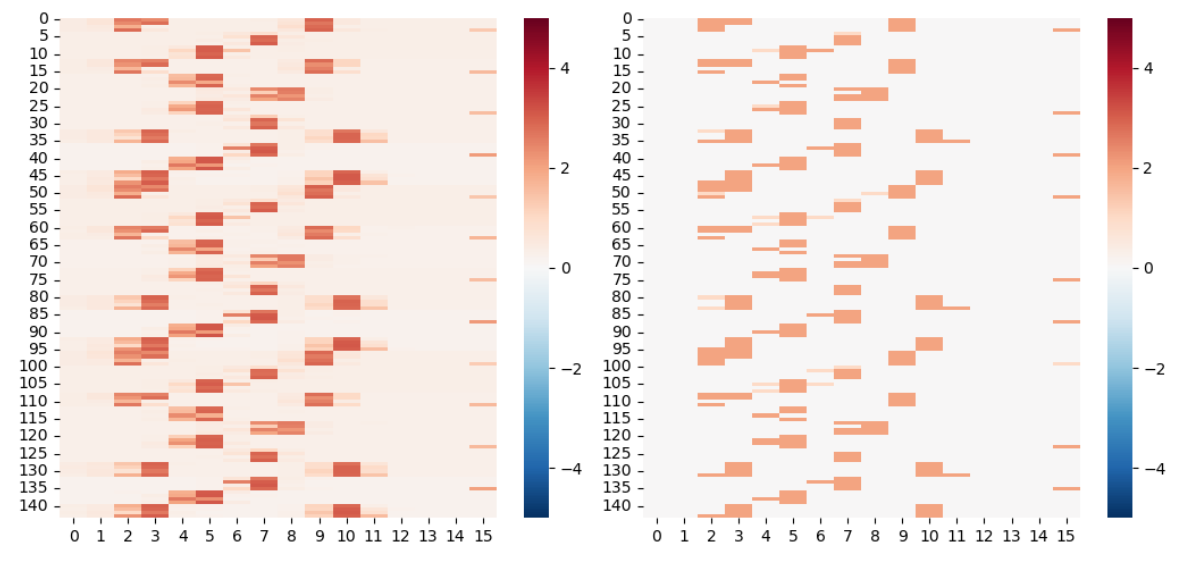
\includegraphics[width=.8\linewidth]{img/chapter5/temporal_pattern_receptive_fields.png}
    \caption[Receptive fields of the readout neurons showing overlapping temporal patterns]{Precise (on the left) and quantized (on the right) matrices showing the formed receptive fields of the readout neurons over the neural sheet of 3 delay lines, after the training on four different 4-step patterns. The X and Y axes are the weight values coming from presynaptic neurons, organized as a continuous sheet: X-axis indices follow the delay line (each new column is the next cluster), Y-axis indices are sorted such that the weights are grouped per each readout neuron.}
  \label{fig:temporal_pattern_receptive_fields}
\end{figure}

Each readout cluster had 3 neurons, so each in the matrix, every pattern is encountered 3 times.

In the inference, the pattern recognition accuracy was around 80\%. However, this number cannot be characteristic of the task as, due to mismatch, usually the 3 classes out of 4 had perfect 100\% recognition rate with only one of them being continuously mislabeled.

From the receptive field illustration, one might see the reason for that. The bottleneck of this architecture is the readout sensitivity. Multiple settings are possible, and since this design is in the phase of ongoing research, we would not claim which one is the best.

One option is to set the firing thresholds of the readout neurons very high, such that only spikes from all correct delay line clusters would arrive at (almost) the same time. Specifically, it means that with 4 coincidental spikes the readout neuron should fire, but with one less input spike it should remain silent. This is needed to spot the difference between patterns that differ only by one value. Some preliminary tests showed that this is possible, especially if multiple readout neurons learn the same class (i.e. the readout clusters are larger than size 1). This helps overcoming the on-chip variability of the neuron thresholds and excitabilities.
Obviously, this approach does not scale well with pattern length, as each additional step in the sequence is one more coincidental input, making it the readout firing thresholds incredibly difficult to configure. Coincidence detection, however, is not new to neuromorhic systems: Nicoletta Risi characterized it extensively for her stereo-vision setup~\cite{Risi_etal21}, and Moritz Milde with Germain Haessig and colleagues demonstrated its viability for touch localization~\cite{Haessig_etal20}.

Alternatively, a rate-based readout is possible by turning the thresholds of the readout neurons down and increasing their both gain and EPSP amplitudes and lengths. This would result in the readout neuron responding with a burst to the correct coincidence of the arriving EPSPs. The tuning between the EPSP time constant, the readout neuron's time constant and the sequence step interval $\tau_{sep}$ should be matched so that the inputs from consecutive clusters do not overlap. This way, the readout cluster receiving the most activation from the pattern would fire the most and define the class label.\\

\begin{figure}[h!]
  \centering
  \begin{subfigure}{0.22\textwidth}
    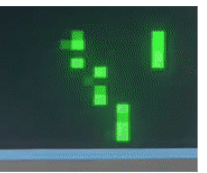
\includegraphics[width=\linewidth]{img/chapter5/pattern_3213.png}
    \caption{}
  \end{subfigure}
  \begin{subfigure}{0.22\textwidth}
    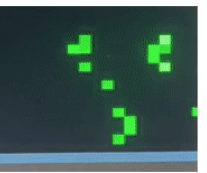
\includegraphics[width=\linewidth]{img/chapter5/pattern_3213_2.png}
    \caption{}
  \end{subfigure}
  \begin{subfigure}{0.22\textwidth}
    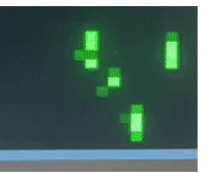
\includegraphics[width=\linewidth]{img/chapter5/pattern_3213_3.png}
    \caption{}
  \end{subfigure}
  \begin{subfigure}{0.22\textwidth}
    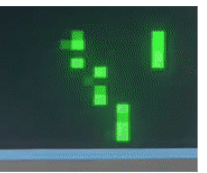
\includegraphics[width=\linewidth]{img/chapter5/pattern_3213_4.png}
    \caption{}
  \end{subfigure}
    \caption[Temporal pattern versions in the DYNAP-SE1 interface]{Multiple presentations of the same temporal pattern $[1,2,3,1]$ in the DYNAP-SE1 interface, moving along the delay lines. Each pixel represents a neuron and is illuminated when the neuron fires. The vertical bars are the pulses traveling from the left to the right along the delay lines. Variability can be seen in the activations of neurons, both in timing and intensity. However, the clustering of the neurons results in equal spacing between the inputs despite the variability of the individual silicon circuits, demonstrating temporal averaging.}
  \label{fig:temporal_patterns_on_dynapse}
\end{figure}

One of the big surprising findings in this series of experiments was the fact that despite the variability of individual neurons and synapses, the propagation speed of the pulses remained constant. In Figure~\ref{fig:temporal_patterns_on_dynapse} it can be seen through the fact that the spacing between the pulses remains the same across multiple presentations. It is visible that activation of the single neurons is inhomogenous, as some neurons just do not fire within the clusters of 4, or some neurons fire before or after the rest of the majority representing that pulse. We can say that space averaging in this scenario led to \emph{temporal} averaging. A similar observation was done for coupled oscillators (e.g. delay lines looped to themselves) in the work of Renate Krause~\cite{Krause_etal21}.

Interestingly, in both delay lines and coupled oscillators, only one shared parameter (i.e. bias) change is enough to control the speed of the pulse propagation. Indeed, we were able to change the speed (and thus the spacing) between the pulses in the delay lines with just the weight of the excitatory synapses used for feedforward connections.

The speed of activity propagation directly defines its memory capacity and time resolution. The faster the pulses move, the more spaced along the lines they are, but the shorter is the time sequence that can be stored. With slower pulse speed, the memory capacity is increased at the price of time precision.\\


This network has multiple major limitations, opening paths for future work. First, for the current decoding technique to work, all presented sequences have to contain the exact same number of pulses. They might be slightly variable in the lengths of inter-pulse intervals, but the number of coincident pulses at the readout for every pattern has to be the same. Otherwise, some false positives are possible. Second, the network works with temporal binary pulses (like the ones arriving from other neurons upstream), but not slow-evolving time-continuous signals, such as EEG or ECG, which are some of the most popular signal types for pattern spotting. Third, this classification approach would fail to recognize of the same pattern is sped up or slowed down. In training, the slow and the fast versions would be recognized as separate classes. Finally, more work has to be done simply to figure out the correct configuration for readout robustness in its current form. Perhaps some form of disinhibition could help, such that the last cluster in each delay line disinhibits the readout, automatically aligning the patterns within the connectivity matrix, removing the need for the precise timing of the teacher signal.\\

Overall, this network is a principle demonstration of how overlapping temporal sequences can at least be technically classified with inhomogeneous hardware neurons and without any variable synaptic delays.

%\dz{matrix sparsity, zero noise tolerance}

\newpage
\section{Discussion and outlook}

All of the networks we discussed share the same basis constraints. They use spiking deterministic leaky integrating (low-pass-filtering) neurons (with a degree of noise and variability) and ``pulse-extender'' synapses with adjustable but heavily quantized weights. This set of tools might feel really limiting compared to the freedom of digital simulations, but (and this is debatable) this limiting factor can be seen as a way to focus the research. While the networks of the brain have much more intricate not only electrical but also chemical machinery, even our unpretentious set of elements was able to capture computational principles of different domains.\\

\subsection{Unused neural mechanism: Firing threshold adaptation}

In fact, we still did not utilize the adaptive firing threshold mechanism of the DYNAP-SE1 neurons, which would introduce another filtering stage on top of the mechanisms discussed. Depending on the threshold relaxation time constant setting, this additional activity-based negative feedback loop at a neuron level could serve various functions in the structures we have shown. Basically, our low-pass filtering neurons would let transients through, meaning that any changes in our steady firing activity would be more powerful. In other words, it increases the significance of novelty in the input (or saliency detection). For WTAs, for example, this would result in easier state or population code change once the input changes. This mechanism generally enables \ac{SSA} in models for saliency detection in various steady or rhythmic continuous input streams~\cite{Nelken_Chechik07, Vanattou-Saifoudine_etal21}. The work of Nik Dennler~\cite{Dennler_etal21a} showed how this adaptation of DYNAP-SE1 neurons can be used to filter and detect anomalies in continuous signals.
At the same time, we can expect a decrease in variability in the firing rate responses of the neurons, as the adaptation circuits carry their own mismatch-induced variability profile.

In relation to learning, the homeostatic function of activity adaptation could help dissolve unwanted activity clusters forming through STDP, which is a natural tendency of the correlation-based learning rule. In a setting where a set of plastic connections is targeting a pool of neurons, unrestricted STDP would keep reinforcing the weights toward the already most active neurons. In this work, we addressed this issue with heterosynaptic plasticity by clamping the total input weight to a fixed value; the adaptation could be an alternative to this, decreasing the excitability for the established cluster and giving more chances for the rest of the network to activate.

This relates to the challenge of maintaining the mapping continuity in the experiment from the first section of this chapter. The linear mapping forms independently in different regions of the matrix, recruiting the neighbouring connections. Some regions end up being inverse to the others, and the gaps cannot be eliminated without a symmetry-breaking mechanism. The increase in transient activity, however, would likely not solve this issue, as the changes happen on a very slow timescale. The search for a bio-plausible symmetry-breaking mechanism could be one of the future research directions. This effect, in fact, might be specific to the mapping between defined 1D attractors; if the neighbouring neurons in postsynaptic population are arranged in 2D, the neurons with the close receptive fields in the 1D input layer can be arranged continuously (see orientation selectivity maps in visual cortex~\cite{Ferster_Miller00, Mariño_etal05}).\\

%\dz{Exploration: from the stochastisity of the matrix updates}

%\dz{Point: effect of clustering - still applies. Even in for the temporal propagation}

%\dz{Point: proved that the approach with a PPU (or EPC) works well an can be used further}

%\dz{Coincidence detection as a main spike-based implementation constraint}

%\dz{Point: we still did not fully go intro the reinforcement learning yet, we barely scratched the surface}


%\dz{Importance of running experiments with self-forming metric within input and output. Now that the architecture is in place, this should be doable.}


%\dz{This should be tested for keyword detection task in the flow of data or arrhythmia detection, REF Mosaic}


%\dz{Closed setup points: hard to make it work in HW. Needs a step back to simulations and the network itself. FIND REFS? the network architecture should be different. The setup was not a limiting factor... we did not really go intro the aspects of reinforcement learning at all.}

\subsection{Internal reward generation}

Finally, one of the ideas that this work got close to but has not covered is the internal generation of the reward signal. The reward-modulated STDP plasticity rule chosen in Chapter~\ref{ch:dynamic_connectome} models the presence of the global change in extracellular dopamine concentration~\cite{Izhikevich07} but does not assume any origin of that signal. In the brain, the \ac{VTA} contains dopaminergic neurons and is responsible for the reward prediction error\cite{WatabeUchida_etal17}. One of the interesting modeling tasks would be to have the role of the dopaminergic neurons taken by the actual physical on-chip ones within a coherent closed-loop architecture. I propose an idea of what such architecture could look like, inspired by the concepts of relational networks, belief propagation networks and networks of distributed controllers~\cite{Diehl_Cook16, Jug12}.

Now that at the end of Chapter~\ref{ch:static_networks}, we have implemented relational networks as a computational primitive that is capable of storing a map between multiple inputs, we could use it in a way that produces an error signal. If we use an $A+B=C$ relation shown in Figure~\ref{fig:rel_net} (and reverse it to $A-C=B$), we could encode an error between two one-dimensional variables. Those variables could be the expected state of the agent, given by an internal world model, and the actual perceived agent state from a sensor. Building on this, we can construct a network of variable-encoding populations bidirectionally connected with 3-way relational maps.

\begin{figure}[h!]
  \centering
     \begin{subfigure}{.9\textwidth}
    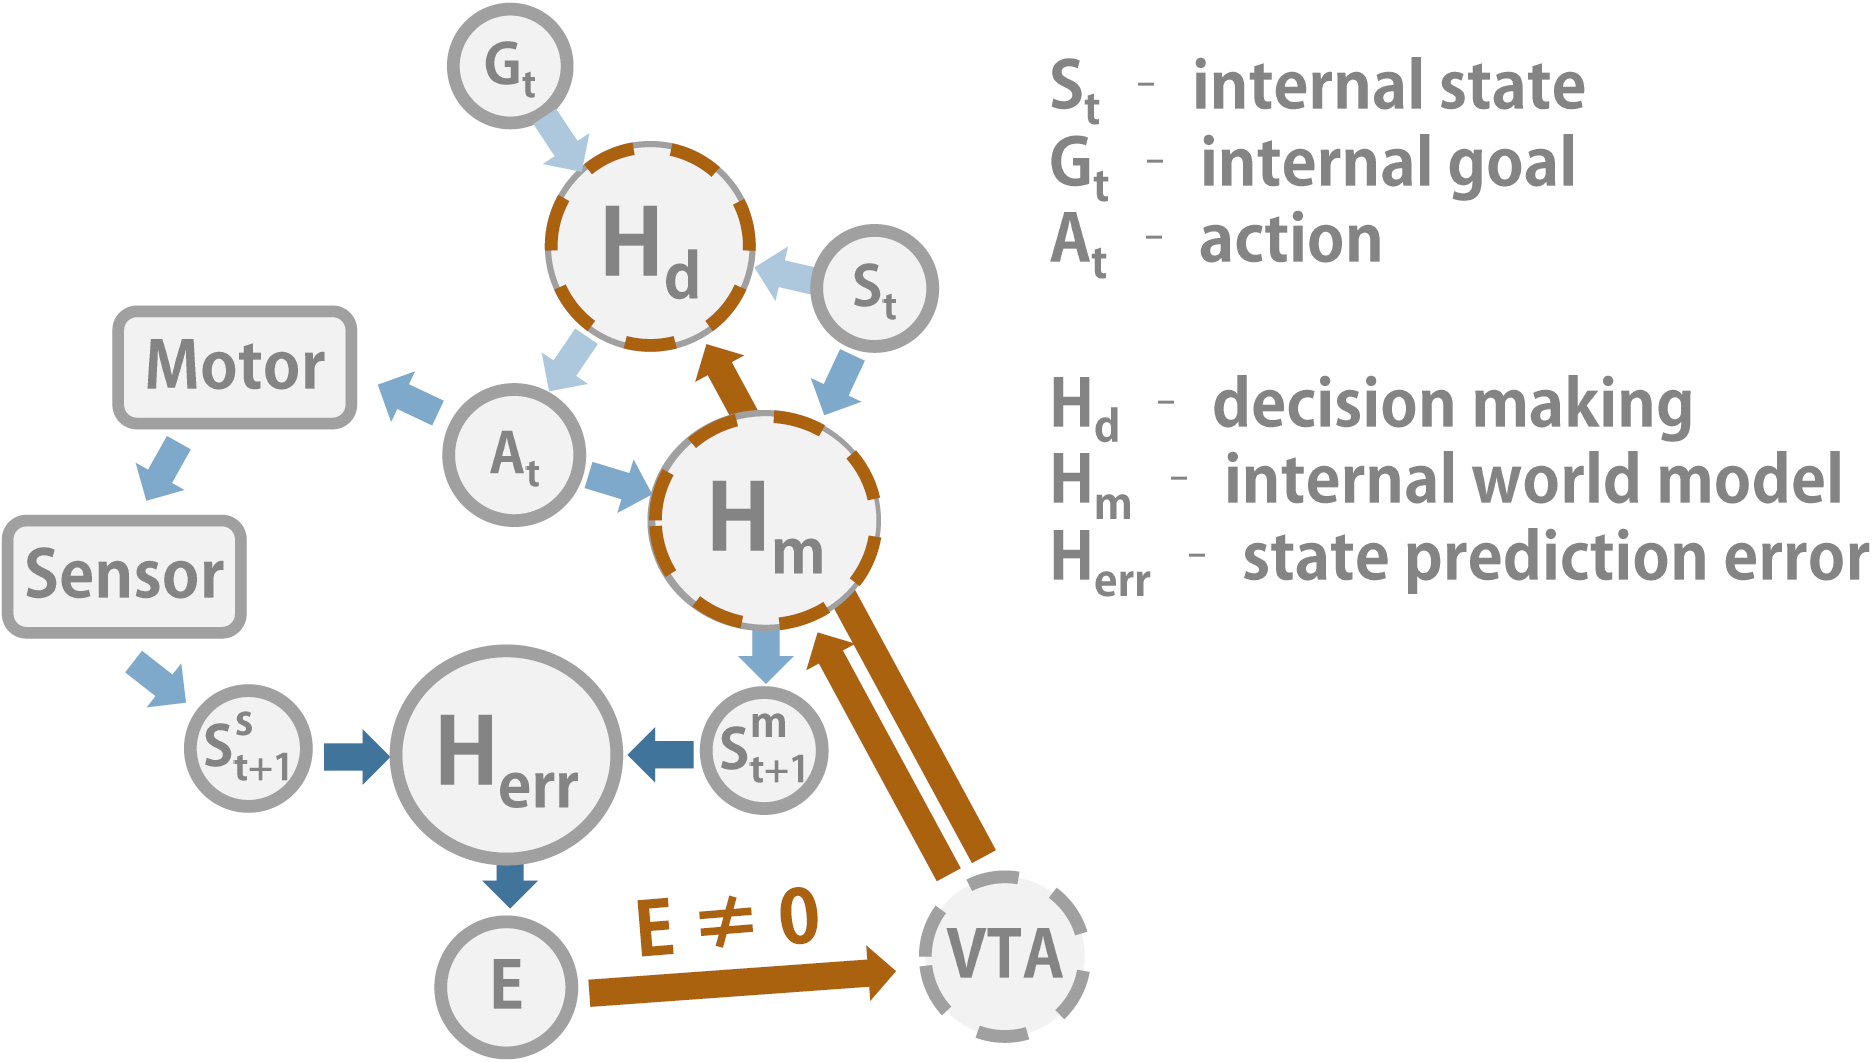
\includegraphics[width=\linewidth]{img/chapter5/Internal_reward_generation_in_a_relnet_a.png}
    \caption{Plasticity triggering pathway}
    \label{fig:forward_pass}
    \end{subfigure}\\
    \begin{subfigure}{.9\textwidth}
    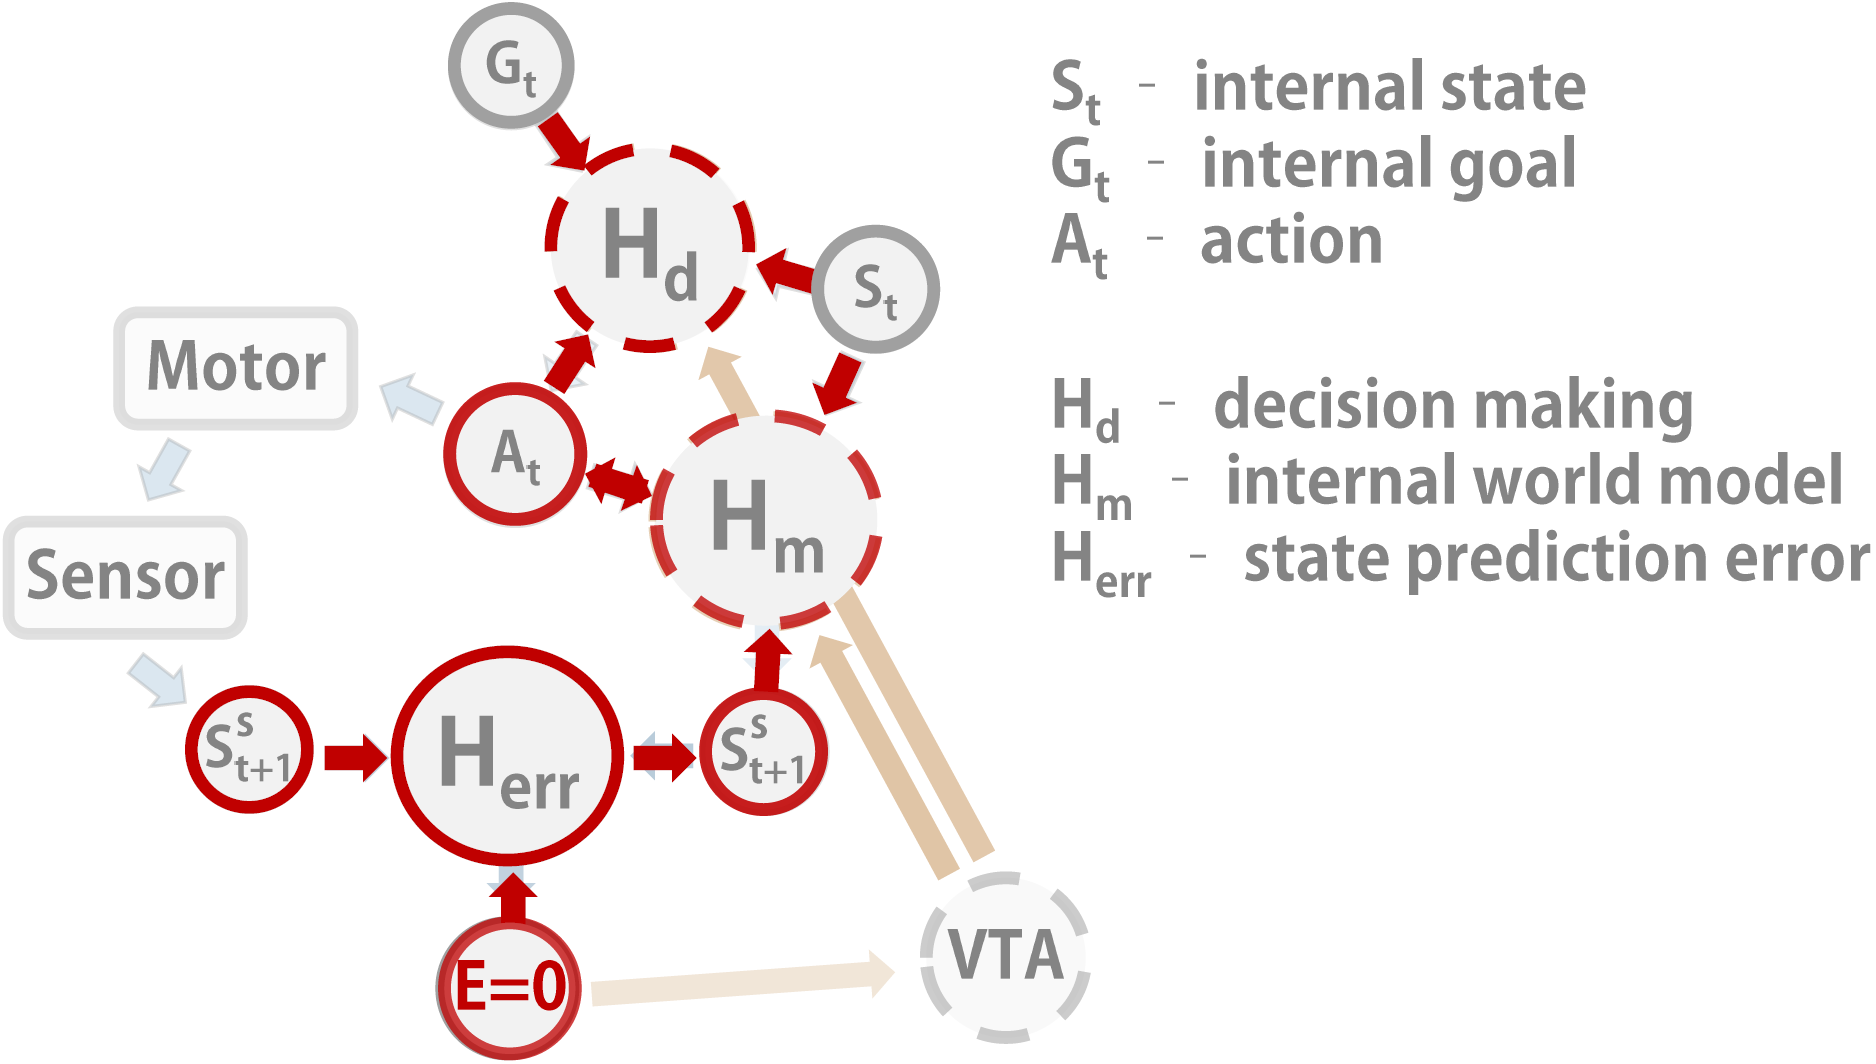
\includegraphics[width=\linewidth]{img/chapter5/Internal_reward_generation_in_a_relnet_b.png}
    \caption{Updated activation pathway}
    \label{fig:return_pass}
  \end{subfigure}
  \centering
    \caption[Internal reward generation in a relational network]{A sketch of a relational network for a model-based reinforcement learning agent with internal reward generation.}
  \label{fig:internal_reward_generation_in_a_relnet}
\end{figure}


Figure~\ref{fig:internal_reward_generation_in_a_relnet} introduces a preliminary sketch of a relational network that implements a model-based reinforcement learning agent operating in a discrete state space $S$. Being in the state $S_t$ at a time $t$ and having some defined objective goal $G_t$, it is taking an action $A_t$ to make the next state $S_{t+1}$ closer to the goal. The network would have three 3-way relations: $H_d$ is the policy network that defines which action should be taken given the state; $H_m$ is the model that predicts the next state $S_{t+1}$ given the action and the current state; $H_{err}$ the prediction error detector that, based on the predicted state $S^m_{t+1}$ and the ground truth received from the environment $S^s_{t+1}$, generates and error signal $E$. The network, however, is by no means complete and assumes some additional inputs or mechanisms. For instance, some of the relations might have to be fully inhibited in some stages of the network function.

The idea is to try to utilize the bidirectionality of connections in a relational network. We propose at least two passes of information for every step of the agent.

\emph{Forward pass} (Figure~\ref{fig:forward_pass}): Once the action $A_t$ is taken, it is translated both to the world model $H_m$ and the Motor that takes an action in the real environment. The Sensor returns the updated state $S^s_{t+1}$. The model $H_m$, given the action and the current state, makes its own prediction $S^m_{t+1}$. The prediction error block calculates the error which is projected to population $E$. Now, activity in this population $E$ can activate the model VTA population, either instantly or with some delay, or any other kind of gating. Activity in VTA would be detected by the plasticity controller framework as a reward signal, activating plasticity in maps $H_d$ or $H_m$, which is yet to be designed.

\emph{Backwards pass (Figure~\ref{fig:return_pass})}: Once the error-based reward signal is sent, the backward pass can begin with clamping the error signal to $E=0$. This would force the $H_{err}$ map to change the encoded predicted state to become equal to the ground truth $S^m_{t+1}:=S^s_{t+1}$. This is where the learning sequence get vague. One of the options is to update the world model map $H_m$, so that the pair $[S_t, A_t]$ produces the correct prediction. Another option would be to try and update the policy network $H_d$ given the pair $[S^s_t+1, S_t]$. The role of the reward signal is to make either of these maps plastic for some period of time such that the mapping can be updated. After this pass is complete, the ``current'' network state $S_t$ is updated (the connection not shown) according to the output of the sensor and the new step begins.

To reiterate, this is a preliminary idea of a network with many components still undefined. However, I do not see any major impossible operations, and the technical basis for hardware implementation of such a system is now fully available.